\section{Конечнопорождённые абелевы группы}
\begin{remark}
    В данном разделе используется аддитивная терминология: \\
    $(A, +)$ - абелева группа, $\forall a \in A, n \in \Z$:
    \[na = \begin{cases}
        \undermat{n}{a + ... + a}, \ n > 0;\\
        \\
        0, \ a = 0;\\
        \undermat{|n|}{(-a) + ... + (-a)}, \ n < 0
    \end{cases}\] 
\end{remark}
\begin{properties} ($\forall a, b, \in A, \ n, m, \in \Z$)
    \begin{enumerate}
        \item $(n+m)a = na + ma$;
        \item $n(a+b) = na + nb$;
        \item $(nm)a = n(ma)$
    \end{enumerate}
\end{properties}
\begin{proof}
    Непосредственный разбор случаев - знаков $m, n$.
\end{proof}
\begin{definition}
    (Целочисленнной) линейной комбинацией элементов $a_1,...,a_k \in A$ называется выражение $n_1a_1 + ... + n_ka_k \ (n_i \in \Z)$.\\
    Если элемент $b \in A$ равен некоторой линейной комбинации $a_1,...,a_k \in A$, то говорят, что $b$ выражается через $a_1,...,a_k$.
\end{definition}
\begin{definition}
    Система элементов $a_1,...,a_k$ называется линейно зависимой, если $\exists n_1,...,n_k \in \Z$, не все равные 0, такие, что $n_1a_1 + ... + n_ka_k = 0$.\\
    В противном случае система $a_1,...,a_k$ называется линейно независимой.
\end{definition}
\begin{example}
    $A = \Z_3 \oplus \Z_4$. Система из одного элемента $(1, 1)$ - линейно зависима: $12 \cdot (1, 1) = (0, 0)$
\end{example}
\begin{definition}
    Пусть $A$ - абелева группа, $a_1,...,a_k \in A$. \\
    Будем обозначать $\langle a_1,...,a_k \rangle = \{n_1a_1 + ... + n_ka_k \ | \ n_i \in \Z\}$\\
    (для бесконечного числа $a_k$ - всевозможные конечные линейные комбинации)
\end{definition}
\begin{subtheorem}
    $\langle a_1,...,a_k \rangle$ - наименьшая подгруппа $A$, содержащая $a_1,...,a_k$. 
\end{subtheorem}
\begin{proof}
    Пусть $H$ - наименьшая подгруппа, содержащая $a_1,...,a_k$. Тогда с одной стороны $\langle a_1,...,a_k \rangle \subseteq H$ по определению подгруппы, а с другой стороны $\langle a_1,...,a_k\rangle$, очевидно, подгруппа в $A$. Значит, $H = \langle a_1,...,a_k \rangle$ 
\end{proof}
\begin{definition}
    Если $A = \langle a_1,...,a_k \rangle$, то говорят, что $A$ порождается $a_1,...,a_k$. Элементы $a_1,...,a_k$ называются порождающими (образующими).
\end{definition}
\begin{definition}
    Если $\exists$ конечное множество элементов $a_1,...,a_k \in A$, что $A = \langle a_1,...,a_k \rangle$, то $A$ называется конечнопорождённой.
\end{definition}
\begin{examples}\tab
    \begin{enumerate}
        \item $\Q$ - не конечнопорождённая;
        \item $U$ (комплексные корни из 1) - не конечнопорождённая;
        \item $\Z, \Z_n$ - конечнопорождённые (циклические);
        \item $\Z \oplus \Z$ - конечнопорождённая, не циклическая (примеры систем порождающих - $(1, 0), (0, 1)$ или $(3, 0), (4, 5), (0, 1)$) 
    \end{enumerate}
\end{examples}
\begin{definition}
    Линейно независимая система порождающих группы $A$ называется базисом (или свободной системой порождающих).
\end{definition}
\begin{subtheorem} (не было в лекции)\\
    $a_1,...,a_k$ - базис $\Longleftrightarrow$ любой элемент $A$ выражается через $a_1,...,a_k$ единственным образом.
\end{subtheorem}
\begin{proof}
    $ \\ \Longrightarrow: \ \ $ Из определения базиса любой элемент имеет разложение по базису.
    \[\alpha_1e_1 + ... + \alpha_ne_n = a = \alpha_1'e_1 + ... + \alpha_n'e_n \Longrightarrow (\alpha_1 - \alpha_1')e_1 + ... + (\alpha_n - \alpha_n')e_n = 0\] 
    Отсюда из линейной независимости $\alpha_i = \alpha_i' \ \forall i$, т.е. разложение единственно.\\
    $\Longleftarrow: \ \ $ Любой элемент $a \in A$ имеет разложение по $a_1,...,a_n$ - система $a_1,...,a_n$ порождает $A$. Разложение любого элемента единственно $\Longrightarrow 0$ имеет только тривиальное разложение $\Longrightarrow a_1,...,a_n$ линейно независимы. 
\end{proof}
\begin{example}
    $\Z_3 \oplus \Z_4$ - не имеет базиса: любая система элементов в ней линейно зависима ($12 \cdot a = 0 \ \forall a \in A$).
\end{example}
\begin{definition}
    Конечнопорождённая абелева группа, имеющая базис, называется свободной абелевой группой.
    По определению $A = \{0\}$ - свободная абелева группа.
\end{definition}
\begin{example}
    $\Z^n = \undermat{n}{\Z \oplus ... \oplus \Z}$ - свободная абелева группа; $\\ \\$
    Базис - $(1,0,...0), (0, 1,...,0),...,(0,0,...,1)$. Проверим это:
    \begin{enumerate}
        \item Линейная независимость:
        \[\alpha_1e_1 + ... + \alpha_ne_n = 0 \Longrightarrow (\alpha_1,...,\alpha_n) = (0,...,0) \Longrightarrow \alpha_i = 0 \ \forall i\]
        \item Порождаемость группы:
        \[\forall a \in \Z^n: a = (a_1,...,a_n) = a_1e_1 + ... + a_ne_n\]
    \end{enumerate}
\end{example}
\begin{lemma} (Основная лемма о линейной зависимости для абелевых групп)\\
    Если абелева группа $A$ обладает базисом из $n$ элементов, то любая система из $m > n$ элементов линейно зависима.
\end{lemma}
\begin{proof}
    Пусть $e_1,...,e_n$ - базис группы $A$, $a_1,...,a_m \in A$ - произвольные элементы. Тогда из определения базиса:
    \[\begin{cases}
        a_1 = \alpha_{11}e_1 + ... + \alpha_{1n}e_n \longrightarrow (\alpha_{11}, ..., \alpha_{1n})\\
        $\vdots$ \\
        a_m = \alpha_{m1}e_1 + ... + \alpha_{mn}e_n \longrightarrow (\alpha_{m1}, ..., \alpha_{mn})
    \end{cases}\]
    Строки $\overline{\alpha}_i = (\alpha_{i1}, ..., \alpha_{in})$ можно рассматривать как векторы из пр-ва $\Q^{n}$ над $\Q$. Так как $m > n$, по ОЛЛЗ для векторных пространств система $\overline{\alpha}_1,...,\overline{\alpha}_m$ линейно зависима, т.е. $\exists \lambda_1,...,\lambda_m \in \Q$, не все равные нулю, что $\lambda_1\overline{\alpha}_1 + ... + \lambda_m\overline{\alpha}_m = 0$.\\
    Тогда если $d$ - НОК знаменателей ненулевых $\lambda_i$, то $(d\lambda_1)\overline{\alpha}_1 + ... + (d\lambda_m)\overline{\alpha}_m = 0$ - нетривиальная целочисленная линейная комбинация, равная нулю.\\
    Тогда $(d\lambda_1)a_1 + ... + (d\lambda_m)a_m = 0$, т.е. $a_1,...,a_m$ линейно зависимы.
\end{proof}
\begin{theoremnum}
    Все базисы свободной абелевой группы $A$ равномощны.
\end{theoremnum}
\begin{proof}
    Очевидно следует из ОЛЛЗ для абелевых групп.
\end{proof}
\begin{definition}
    Число элементов в базисе свободной абелевой группы $A$ называется рангом группы $A$. Обозначается $\textup{rk }A$. По определению $A = \{0\} \Longrightarrow \textup{rk }A = 0$.
\end{definition}
\begin{theoremnum}
    Все свободные абелевы группы ранга $n$ изоморфны между собой (в частности, изоморфны $\Z^n$).
\end{theoremnum}
\begin{proof}
    $ \\$Пусть $A$ - свободная абелева группа, $\textup{rk }A = n$, $e_1,...,e_n$ - базис. Рассмотрим отображение $\phi: A \rightarrow \Z^n$ такое, что $\forall a = \alpha_1e_1 + ... + \alpha_ne_n \in A \ \phi(a) = (\alpha_1,...,\alpha_n)$. Покажем, что $\phi$ - изоморфизм:
    \begin{enumerate}
        \item Биекция - следует из единственности разложения по базису;
        \item Гомоморфизм: пусть $a = \alpha_1e_1 + ... + \alpha_ne_n, b = \beta_1e_1 + ... + \beta_ne_n$. Тогда:
        \[\phi(a + b) = \phi((\alpha_1 + \beta_1)e_1 + ... + (\alpha_n + \beta_n)e_n) = ((\alpha_1 + \beta_1), ...,(\alpha_n + \beta_n)) =\]
        \[ = (\alpha_1,...,\alpha_n) + (\beta_1,...,\beta_n) = \phi(a) + \phi(b)\]
    \end{enumerate}
    Отсюда $A \simeq \Z^n$.\\
    Если $\textup{rk }A = \textup{rk }B = n$, то $A \simeq \Z^n \simeq B \Longrightarrow A \simeq B$.
\end{proof}
\begin{theoremnum}
    Любая подгруппа $B$ свободной абелевой группы $A$ ранга $n$ является свободной абелевой, причём $\textup{rk }B \leqslant n$.
\end{theoremnum}
\begin{proof}
    Случай $n = 0$ очевиден. Индукция по $n$:\\
    \tab База: $n = 1 \Longrightarrow A \simeq \Z \Longrightarrow A = \langle e \rangle$.\\
    Знаем, что любая подгруппа циклической группы - циклическая.\\
    Пусть $B = \langle ke \rangle, k \in \N \cup \{0\}$. Тогда:
    \[k = 0 \Longrightarrow B = \{0\} \Longrightarrow \textup{rk }B = 0 < 1 = \textup{rk }A\]
    \[k \neq 0 \Longrightarrow B = \langle ke \rangle \simeq \Z \Longrightarrow \textup{rk }B = 1 = \textup{rk }A\]
    \tab Шаг: пусть $e_1,...,e_n$ - базис свободной группы $A$.\\
    Рассмотрим $\tilde{A} = \langle e_1,...,e_{n-1} \rangle \leq A$ - свободная абелева ранга $n-1$.\\
    Рассмотрим $\tilde{B} = B \cap \tilde{A}$ - подгруппу $B$ в $\tilde{A}$. По предположению индукции $\tilde{B}$ - свободная абелева, причём $\textup{rk }\tilde{B} \leqslant \textup{rk }\tilde{A} = n-1$.\\
    Если $B = \tilde{B}$, то теорема доказана. \\
    Иначе рассмотрим гомоморфизм (проекцию на $\langle e_n \rangle$) \\ $\pi: A \rightarrow \Z: \forall a = \alpha_1e_1 + ... + \alpha_ne_n \in A \ \pi(a) = \alpha_n \ (\textup{Ker }\pi = \tilde{A}, \textup{Im }\pi = \Z)$.\\
    Знаем, что $\pi(B)$ - подгруппа в $\Z \Longrightarrow \pi(B) = \langle k \rangle$ ($k \neq 0$ из $B \neq \tilde{B}$).\\
    Рассмотрим $b_0 \in B$ такой, что $\pi(b_0) = k$, т.е. $b_0 = \beta_1e_1 + ... + \beta_{n-1}e_{n-1} + ke_n$. Докажем, что если $b_1,...,b_s$ - базис $\tilde{b}$, то $b_0, b_1,...,b_s$ - базис $B$ (тогда $B$ - свободная абелева, $\textup{rk }B \leqslant n$)
    \begin{enumerate}
        \item Проверим линейную независимость:
        \[\lambda_0b_0 + ... + \lambda_sb_s = 0 \Rightarrow \pi(\lambda_0b_0 + ... + \lambda_sb_s) = 0 \Rightarrow \lambda_0\pi(b_0) + ... + \lambda_s\pi(b_s) = 0 \Longrightarrow\]
        \[\lambda_0k = 0 \Rightarrow \lambda_0 = 0\]
        Линейная комбинация $\lambda_1b_1 + ... + \lambda_sb_s = 0$ тривиальна, так как $b_1,...,b_s$ - базис $\tilde{B}$. Отсюда $b_0,b_1,...,b_s$ линейно независимы.
        \item $\langle b_0,b_1...,b_s \rangle \overset{?}{=} B$:\\
        Рассмотрим произвольный $b \in B$. $\pi(b) \in \langle k \rangle \Longrightarrow \pi(b) = tk, \ t \in \Z$.\\
        Пусть $\tilde{b} = b - tb_0$. Тогда $\pi(\tilde{b}) = \pi(b) - t\pi(b_0) = tk - tk = 0 \Longrightarrow \tilde{b} \in \textup{Ker }\pi = \tilde{A} \Longrightarrow \tilde{b} \in \tilde{A} \cap B = \tilde{B} \Longrightarrow \tilde{b} = t_1b_1 + ... + t_sb_s \Longrightarrow b = tb_0 + t_1b_1 + ... + t_sb_s$.
    \end{enumerate}
\end{proof}
\subsection{Связь между базисами свободной абелевой группы}
\begin{definition}
    Пусть $A$ - свободная абелева группа, $\E = \{e_1,...,e_n\}$, $\tilde{\E} = \{\tilde{e}_1,...,\tilde{e}_n\}$ - базисы $A$.
    \[\begin{cases}
        \tilde{e}_1 = c_{11}e_1 + ... + c_{n1}e_n\\
        \vdots \\
        \tilde{e}_n = c_{1n}e_1 + ... + c_{nn}e_n
    \end{cases} \Longrightarrow (\tilde{e}_1,...,\tilde{e}_n) = (e_1,...,e_n)C, \ C = \begin{pmatrix} c_{11} &\dots&c_{1n} \\ \vdots&\null&\vdots \\ c_{n1} &\dots&c_{nn} \end{pmatrix}\]
    Такая $C \in M_n(\Z)$ называется матрицей перехода от $\E$ к $\tilde{\E}$. 
\end{definition}
\begin{subtheorem}
    $ \\$Пусть $C \in M_n(\Z)$. Тогда $C$ - матрица перехода $\Longleftrightarrow \det C = \pm1$. 
\end{subtheorem}
\begin{proof}
    $ \\ \Longrightarrow: \ \ $Пусть $C$ - матрица перехода от $\E$ к $\tilde{\E}$, $D$ - от $\tilde{\E}$ к $\E$. Тогда:
    \[\begin{cases}
        (\tilde{e}_1,...,\tilde{e}_n) = (e_1,...,e_n)C\\
        (e_1,...,e_n) = (\tilde{e}_1,...,\tilde{e}_n)D
    \end{cases} \Longrightarrow CD = DC = E \Longrightarrow D = C^{-1}\]
    \[\det C \cdot \det D = \det CD = \det E = 1\]
    Так как $C, D \in M_n(\Z)$, $\det C,\det D \in \Z \Longrightarrow \det C = \pm 1$. \\
    $\Longleftarrow: \ \ C \in M_n(\Z), \det C = \pm1$. Рассмотрим некоторый базис $\E = \{e_1,...,e_n\}$ и докажем, что $(\tilde{e}_1,...,\tilde{e}_n) = (e_1,...,e_n)C$ - базис.
    \begin{enumerate}
        \item Проверим линейную независимость:\\
        Если $\lambda_1\tilde{e}_1 + ... + \lambda_n\tilde{e}_n = 0$, то линейная комбинация столбцов $C$ с теми же $\lambda_i$ также равна 0. Из $\det C \neq 0$ столбцы линейно независимы, т.е. $\lambda_i = 0 \ \forall i$.
        \item $\langle \tilde{e}_1...,\tilde{e}_n \rangle \overset{?}{=} A$:\\
        Так как $\det C = \pm 1, \ \exists D = C^{-1} \in M_n(\Z)$ (из формулы явного выражения элементов обратной матрицы элементы $D$ целые) $\Longrightarrow (e_1,...,e_n) = (\tilde{e}_1,...,\tilde{e}_n)D$.\\
        $\forall a \in A$ целочисленно выражается через $e_1,...,e_n$, каждый $e_i$ целочисленно выражается через $\tilde{e}_1,...,\tilde{e}_n \Longrightarrow a$ целочисленно выражается через $\tilde{e}_1,...,\tilde{e}_n$
    \end{enumerate}
\end{proof}
\subsection{Элементарные преобразования свободных абелевых групп}
\begin{definition} (ЭП свободных абелевых групп)\\
    Пусть $A$ - свободная абелева группа, $e_1,...,e_n$ - базис $A$. 
    \begin{itemize}
        \item \textbf{ЭП1}: $\tilde{e}_i = e_i + ke_j, \ i \neq j, k \in \Z; \ \ \ \tilde{e}_s = e_s, \ s \neq i$;
        \item \textbf{ЭП2}: $\tilde{e}_i = e_j; \ \ \ \tilde{e}_j = e_i; \ \ \ \tilde{e}_s = e_s, \ s \neq i,j \ (i \neq j)$;
        \item \textbf{ЭП3}: $\tilde{e}_i = -e_i; \ \ \ \tilde{e}_s = e_s, \ s \neq i$;
    \end{itemize}
    Матрицы перехода при этих ЭП:\\
    ЭП1:
    $$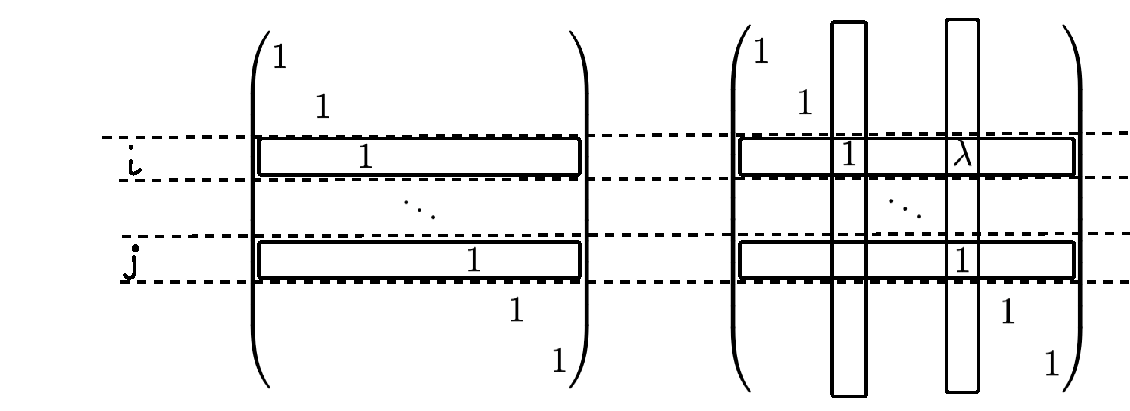
\includegraphics[width=12cm]{image/EP1.pdf}$$
    ЭП2: \tab[6.5cm]:
    $$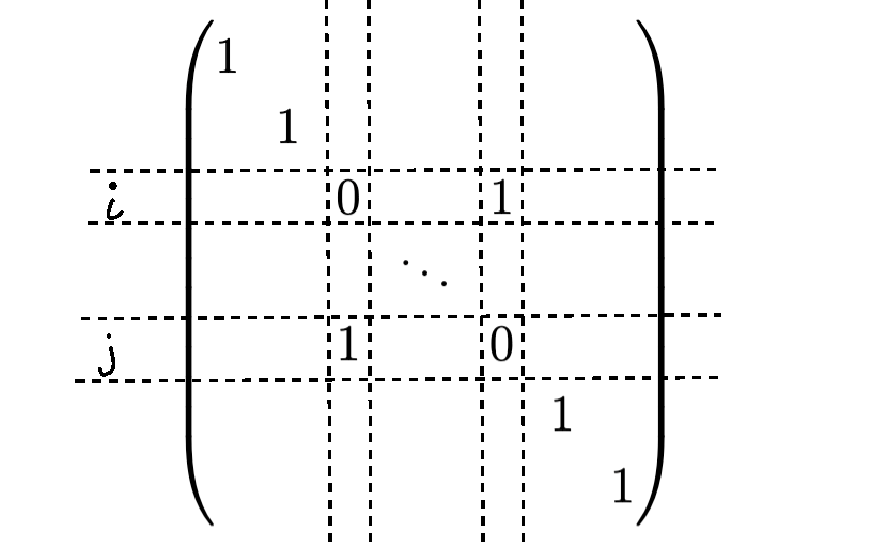
\includegraphics[width=7cm]{image/EP2.pdf}$$
    ЭП3: \tab[5cm] $\begin{pmatrix*}
        1&&&&\\
        &\ddots&&&\\
        &&-1&&\\
        &&&\ddots&\\
        &&&&1
    \end{pmatrix*}$\\
    называются (целочисленными) элементарными матрицами.
\end{definition}
\begin{definition}(ЭП строк целочисленных матриц)
    \begin{itemize}
        \item \textbf{ЭП1}: $\overline{a_i} \to \overline{a_i} + \lambda \overline{a_j}, \ \ i \neq j, k \in \Z$;
        \item \textbf{ЭП2}: $\overline{a_i} \leftrightarrow  \overline{a_j}, \ \ i \neq j$;
        \item \textbf{ЭП3}: $\overline{a_i} \rightarrow (-1) \overline{a_i}$;
    \end{itemize}
\end{definition}
(Аналогично определены ЭП над столбцами матрицы)\\
\textbf{Приведение целочисленной матрицы с помощью целочисленных ЭП к "диагональному" \ виду}\\
Пусть $A = (a_{ij}) \in M_{n \times m}(\Z)$.
Будем говорить, что матрица $A$ имеет "диагональный" \ вид, если либо $A = 0$, либо $a_{ii} = \alpha_i \in \N, i = \overline{1,l}$ и $a_{ij} = 0$ иначе.
\[ A = \begin{pmatrix}
      \begin{smallmatrix}
    \alpha_1&&0\\ &\ddots&\\ 0&&\alpha_l
    \end{smallmatrix}  & \vline  & 0\\
     \hline
       0  \ \ & \vline& 0\\

    \end{pmatrix}\]
\begin{lemma}
    Любую матрицу $M\in M_{n \times m}(\Z)$ за конечное число целочисленных ЭП над строками и столбцами можно привести к "диагональному" виду. 
\end{lemma}
\begin{proof}
    Индукция по $n$ - числу строк матрицы.
    При фиксированном $n$ индукция по $\nu(M)$ - наименьшему по модулю ненулевому элементу $M$. \\
    Если $M=0$, то утверждение доказано, поэтому далее $M \neq 0$.\\
    База индукции: $n=1 \Longrightarrow M = (a_{11},...,a_{1m})$.\\
    \tab База внутренней индукции: $\nu(M) = 1$ - очевидна (если в строке есть 1, то с помощью неё можно занулить все оставшиеся элементы).\\
    \tab Шаг внутренней индукции: Пусть $\nu(M) = |a_{1j}|$. Если $a_{1j} < 0$, то применим ЭП3 к стоблцу $j$; если $j > 1$, то применением ЭП2 поменяем 1-й и $j$-й столбцы местами. После этих операций $\nu(M) = a_{11}$.\\
    $\forall j > 1: a_{1j} = a_{11}q_j + r_j$, где $0 \leqslant r_j < a_{11}$. Вычитая с помощью ЭП1 из $j$-го столбца 1-й, умноженный на $q_j$, получим строку $\tilde{M} = (a_{11}, r_2,...,r_m)$.\\
    Если все $r_j = 0$, то диагональный вид получен, иначе можно воспользоваться предположением индукции ($\nu(\tilde{M}) < \nu(M)$).\\
    Шаг индукции: Пусть $\nu(M) = |a_{ij}|$. Сначала сделаем $a_{ij}$ положительным (ЭП3), затем переставим его в верхний левый угол (ЭП2).\\
    \tab Случай 1: $M = \begin{pmatrix} a_{11}&\vline&0&\dots&0\\ \hline 0&\vline \\ \vdots&\vline&&\text{\LARGE{C}}  \\ 0 & \vline \end{pmatrix}$ - по предположению индукции приводим $C$ к диагональному виду;\\
    \tab Случай 2: $\exists j > 1: a_{1j} \neq 0$. Тогда, аналогично базе индукции, с помощью ЭП1 приводим верхнюю строчку к виду $\forall j > 1: a_{1j} = 0$.\\
    \tab Случай 3: $\exists j > 1: a_{j1} \neq 0$ - аналогично случаю 2 (ЭП строк вместо столбцов). 
\end{proof}
\begin{exercise}
    Доказать, что с помощью конечного числа целочисленных ЭП над строками и столбцами \[M \sim \begin{pmatrix}
      \begin{smallmatrix}
    \alpha_1&&0\\ &\ddots&\\ 0&&\alpha_l
    \end{smallmatrix}  & \vline  & 0\\
     \hline
       0  \ \ & \vline& 0\\

    \end{pmatrix}\] 
    где $\alpha_l \mid \alpha_{l-1}, \alpha_{l-1} \mid \alpha_{l-2}, ..., \alpha_2 \mid \alpha_1$.
\end{exercise}
\begin{proof}
    По лемме можем с помощью ЭП привести $M$ к диагональному виду. Индукция по $l$ - числу ненулевых $\alpha$ в диагональном виде:\\
    \tab База: $l = 0, 1$ - очевидно;\\
    \tab Шаг: Из теории чисел знаем, что для чисел $\alpha_1, \alpha_i$ существуют $a, b \in \Z$, что $a\alpha_1 + b\alpha_i = d_i =$ НОД($\alpha_1, \alpha_i$). Значит, с помощью ЭП1 можно сделать $a_{1i} = d_i$. Тогда следующими операциями:
    \[\begin{pmatrix}
    \alpha_1&\cdots&0&\cdots&0\\ &\ddots&&&\\ 0&&\alpha_i&&0\\ &&&\ddots&\\0&&&&\alpha_l
    \end{pmatrix} \sim \begin{pmatrix}
    \alpha_1&\cdots&d_i&\cdots&0\\ &\ddots&&&\\ 0&&\alpha_i&&0\\ &&&\ddots&\\0&&&&\alpha_l
    \end{pmatrix} \sim \begin{pmatrix}
    \alpha_1&\cdots&d_i&\cdots&0\\ &\ddots&&&\\ k\alpha_1&&0&&0\\ &&&\ddots&\\0&&&&\alpha_l
    \end{pmatrix} \sim\]
    \[\sim \begin{pmatrix}
    0&\cdots&d_i&\cdots&0\\ &\ddots&&&\\ k\alpha_1&&0&&0\\ &&&\ddots&\\0&&&&\alpha_l
    \end{pmatrix} \sim \begin{pmatrix}
    k\alpha_1&\cdots&0&\cdots&0\\ &\ddots&&&\\ 0&&d_i&&0\\ &&&\ddots&\\0&&&&\alpha_l
    \end{pmatrix}\]
    можем сделать так, чтобы $\alpha_i \mid \alpha_1$. Причём $\alpha_1$ при этих операциях домножается на $k \in \Z$, а значит, делимость на все предыдущие $\alpha_j$ сохраняется. Тогда за $l-1$ таких наборов операций можно сделать $\alpha_1$ общим кратным всех $\alpha$, а матрица без первой строки и первого столбца приводится к нужному виду по предположению индукции.
\end{proof}
\begin{example}
    $(12, 10, 6) \sim (6, 10, 12) \sim (6, 4, 0) \sim (4, 6, 0) \sim (4, 2, 0) \sim (2, 4, 0) \sim (2, 0, 0)$.\\
    (По сути - обобщённый алгоритм Евклида, остаётся НОД чисел 12, 10 и 6).
\end{example}
\setcounter{thcount}{0}
\subsection{Согласованные базисы свободной абелевой группы и её подгруппы}
\begin{theoremnum}
    $ \\$Пусть $A$ - свободная абелева группа ранга $n, B \leq A$ - подгруппа ранга $m$.\\
    Тогда $\exists$ базисы $\tilde{e}_1,...,\tilde{e}_n$ группы $A$ и $\tilde{f}_1,...,\tilde{f}_m$ подгруппы $B$ такие, что \\ $\tilde{f}_i = \alpha_i\tilde{e}_i, \ \alpha_i \in \N$.
\end{theoremnum}
\begin{proof}
    Пусть $e_1,...,e_n$ и $f_1,...,f_n$ - некоторые базисы $A$ и $B$ соответственно. Так как $f_i \in A$, $(f_1,...,f_m) = (e_1,...,e_n)C$, где $C \in M_{n\times m}(\Z)$.\\
    Если $\tilde{f}_1,...,\tilde{f}_m$ - другой базис $B$, то $(f_1,...,f_m) = (\tilde{f}_1,...,\tilde{f}_m)T$, где $T \in M_{n\times n}(\Z)$\\
    Если $\tilde{e}_1,...,\tilde{e}_n$ - другой базис $A$, то $(e_1,...,e_n) = (\tilde{e}_1,...,\tilde{e}_n)S$, где $S \in M_{m\times m}(\Z)$ ($\det T, S = \pm 1$).
    Отсюда
    \[(\tilde{f}_1,...,\tilde{f}_m)T = (\tilde{e}_1,...,\tilde{e}_n)SC \Longrightarrow (\tilde{f}_1,...,\tilde{f}_m) = (\tilde{e}_1,...,\tilde{e}_n)\tilde{C}, \ \ \tilde{C} = SCT^{-1}\]
    Тогда если $S, T^{-1}$ - элементарные матрицы, то $SC$ - ЭП над строками $C$, а $CT^{-1}$ - ЭП над столбцами $C$.
    По лемме 1 $C$ с помощью ЭП можно привести к виду $\tilde{C} = \begin{pmatrix} \begin{smallmatrix}
    \alpha_1&&0\\ &\ddots&\\ 0&&\alpha_m
    \end{smallmatrix} \\\hline 0\end{pmatrix}$ (нулей среди $\alpha_i$ не будет, т.к. векторы базиса $f$ ЛНЗ).
    Отсюда и получаем требуемое равенство $\tilde{f}_i = \alpha_i\tilde{e}_i, \ \alpha_i \in \N$.
\end{proof}
\begin{theorem} (не было в лекции)\\
    Пусть $G = G_1 \times ...\times  G_s$, $H = H_1 \times ...\times  H_s$, причём $H \subseteq G$ и $H_i \unlhd G_i$.\\
    Тогда $H \unlhd G$ и $G/H = G_1/H_1 \times ... \times G_s/H_s$.
\end{theorem}
\begin{proof}
    $ \\$Будем работать с внешним прямым произведением. Рассмотрим отображение
    \[\phi: G \rightarrow G_1/H_1 \times ... \times G_s/H_s\]
    \[\phi(g_1,...,g_s) = (g_1H_1,...,g_sH_s)\]
    $\phi$ - гомоморфизм, так как по $i$-й компоненте $\phi$ реализует естественный гомоморфизм $G \rightarrow G/H_i$.\\
    Ядро $\phi$ - наборы $(g_1,...,g_s)$, которые отображаются в нейтральный элемент, т.е. в $(H_1,...,H_s)$. Получаем
    \[\phi(g_1,..., g_s) = (H_1,..., H_s) \Longleftrightarrow g_i \in H_i, \ \forall i = 1,... , s\]
    Таким образом, $\textup{Ker }\phi = H_1\times ... \times H_s$.\\
    Из определения $\phi$ очевидна сюръективность, т.е. $\textup{Im }\phi = G_1/H_1 \times ... \times G_s/H_s$, а значит, из теоремы о гомоморфизме получаем необходимое утверждение. 
\end{proof}
\begin{remark}
    Для абелевых групп из теоремы получим следующее утверждение: 
    Пусть $A = A_1 \oplus ... \oplus A_n$, $B \leq A$, $B = B_1 \oplus ...\oplus B_n$.\\
    Тогда $A/B = (A_1 \oplus ... \oplus A_n)/(B_1 \oplus ...\oplus B_n) \simeq A_1/B_1 \oplus ...\oplus A_n/B_n$
\end{remark}
\begin{consequensenum}
    В условиях теоремы 1:
    \[A/B \simeq \Z_{\alpha_1} \oplus ... \oplus \Z_{\alpha_m} \oplus \undermat{n-m}{\Z\oplus ... \oplus \Z}\]
    \tab
\end{consequensenum}
\begin{proof}
    По теореме 1: $\tilde{f}_1 = \alpha_1\tilde{e}_1,...,\tilde{f}_m = \alpha_m\tilde{e}_m$.
    \[A = \langle \tilde{e}_1 \rangle \oplus ... \oplus \langle \tilde{e}_m \rangle \oplus \langle \tilde{e}_{m+1} \rangle \oplus ... \oplus \langle \tilde{e}_n \rangle; \ \ B = \langle \alpha_1\tilde{e}_1 \rangle \oplus ... \oplus \langle \alpha_m\tilde{e}_m \rangle \oplus \langle 0 \rangle \oplus ... \oplus \langle 0 \rangle\]
    Тогда из замечания выше:
    \[A / B \simeq \langle \tilde{e}_1 \rangle / \langle \alpha_1\tilde{e}_1 \rangle \oplus ... \oplus \langle \tilde{e}_m \rangle / \langle \alpha_m\tilde{e}_m \rangle \oplus \langle \tilde{e}_{m+1} \rangle / \langle 0 \rangle \oplus ... \oplus \langle \tilde{e}_n \rangle / \langle 0 \rangle \simeq\]
    \[\simeq \Z_{\alpha_1} \oplus ... \oplus \Z_{\alpha_m} \oplus \undermat{n-m}{\Z\oplus ... \oplus \Z}\]
\end{proof}
\begin{consequensenum}
    В условиях теоремы 1: $\textup{rk } A = \textup{rk } B \Longleftrightarrow |A : B| < \infty$.
\end{consequensenum}
\begin{proof}
    По определению $|A : B| = |A/B|$. \\
    Из следствия 1 видно, что если $\textup{rk } A = \textup{rk } B$, то $A/B \simeq \Z_{\alpha_1} \oplus ... \oplus \Z_{\alpha_n}$, и $|A/B| < \infty$, а иначе в прямой сумме встретится слагаемое $\Z$, то есть найдётся элемент бесконечного порядка.
\end{proof}
\begin{subtheoremnum}(Универсальное свойство абелевой группы)\\
    Пусть $S = \{a_1,...,a_n\}$ - система порождающих абелевой группы $A$.\\
    Тогда следующие утверждения эквивалентны:
    \begin{enumerate}
        \item $A$ - свободная с базисом $S$;
        \item $\forall$ абелевой группы $D$, $\forall \ d_1,...,d_n \in D \ \exists!$ гомоморфизм $\phi: A\rightarrow D$ т.ч. $\phi: a_i \mapsto d_i \  \forall i$. 
    \end{enumerate} 
\end{subtheoremnum}
\begin{proof}
    $ \\ 1 \Longrightarrow 2:$  $S$ - базис $A \Longrightarrow \forall a \in A \ \exists! \alpha_i  \in \Z : a = \alpha_1a_1 + ... + \alpha_na_n$.\\
    Рассмотрим отображение $\phi: A \rightarrow D$, заданное как $a = \alpha_1a_1 + ... + \alpha_na_n \mapsto \alpha_1d_1 + ... + \alpha_nd_n$. Оно корректно вследствие единственности разложения по базису, а также очевидно является гомоморфизмом с нужным свойством.\\
    $2 \Longrightarrow 1$. Рассмотрим свободную группу $D$ ранга $n$, в ней рассмотрим базис $d_1,...,d_n$. По условию $\exists!$ гомоморфизм $\phi: A \rightarrow D$, причём $a_i \mapsto d_i$.\\
    Предположим, что $a_1,...,a_n$ линейно зависимы. Тогда \[\lambda_1a_1 +...+\lambda_na_n = 0 \Longrightarrow \phi(\lambda_1a_1 +...+\lambda_na_n) = \lambda_1d_1 +...+\lambda_nd_n = 0\] 
    Противоречие с линейной независимостью $d_1,...,d_n$. Значит, $a_1,...,a_n$ - базис.
\end{proof}
\begin{consequensenum}
    Любая конечнопорождённая абелева группа изоморфна свободной абелевой группе по некоторой её подгруппе $B$.
\end{consequensenum}
\begin{proof}
    Пусть $D = \langle d_1,...,d_n \rangle$. Рассмотрим свободную абелеву группу $A$ ранга $n$ с базисом $a_1,...,a_n$. \\
    По утверждению 1 $\exists$ гомоморфизм $\phi: A \rightarrow D$ такой, что $\phi(a_i) = d_i$.\\
    Из порождаемости гомоморфизм сюръективен, а значит, по теореме о гомоморфизме $D = \textup{Im }\phi \simeq A/\textup{Ker }\phi$, где $\textup{Ker }\phi \leq A$. 
\end{proof}
\begin{consequensenum}
    Любая конечнопорождённая абелева группа раскладывается в сумму циклических подгрупп.
\end{consequensenum}
\begin{proof}
    $D \simeq A/B \simeq \Z_{\alpha_1} \oplus ... \oplus \Z_{\alpha_m} \oplus \undermat{n-m}{\Z\oplus ... \oplus \Z}\\$
\end{proof}
\begin{consequensenum}
    Любая конечнопорождённая абелева группа $D$ раскладывается в прямую сумму конечной абелевой группы и свободной абелевой группы. 
\end{consequensenum}
\begin{proof}
    $D \simeq (\Z_{\alpha_1} \oplus ... \oplus \Z_{\alpha_m}) \oplus \Z^{n-m}$
\end{proof}
\begin{definition}
    Группа, в которой каждый неединичный элемент имеет бесконечный порядок, называется группой без кручения.
\end{definition}
\begin{exercise}
    Если $A$ - свободная абелева, то $A$ - без кручения.
\end{exercise}
\begin{proof}
    Предположим, что $b \in A$ - элемент конечного порядка $m$. По определению свободной группы $b = \alpha_1a_1 + ... + \alpha_na_n$, причём не все $\alpha_i$ равны 0. Тогда $m\alpha_1a_1 + ... + m\alpha_na_n = mb = 0$ - противоречие с линейной независимостью базиса.
\end{proof}
\begin{consequensenum}
    Если $A$ - конечнопорождённая абелева группа без кручения, то $A$ - свободная абелева группа.
\end{consequensenum}
\begin{proof}
    В обозначениях следствия 5 $m = 0$.
\end{proof}